\section{Otimização e/ou justificação do desempenho tendo em conta os parâmetros de configuração do PostgreSQL}

\subsection{Configuração do \textit{shared\_buffers}}

O parâmetro de configuração \textit{shared\_buffers} determina a quantidade de memória RAM dedicada ao \textit{PostgreSQL} que vai ser usada para armazenar dados enquanto executa queries.

Inicialmente, podia-se prever que quanto maior fosse a quantidade de memória dedicada melhor seriam os resultados de desempenho esperados. É uma conclusão precipitada, pois o \textit{PostgreSQL} utiliza esta memória para efetuar operações e não para \textit{cache} de disco, por exemplo.

Um valor razoável para para o \textit{shared\_buffers} é de 25\% da memória RAM do sistema (2GB) mas decidiu-se extender os testes até 50\% da memória do sistema (4GB). Apesar de valores acima de 40\% serem, provavelmente, menos eficazes, pois o \textit{PostgreSQL} conta também com a \textit{cache} do sistema operativo.

Para o \textit{benchamark} foram usados valores de memória RAM entre os 128MB, valor por defeito na configuração, e os 4096MB. Os resultados segue na próxima tabela.

\begin{table}[!h]
\center
\small
\begin{tabular}{|c|c|c|c|c|}
\hline
\textbf{\# tamanho (MB)} & \textbf{\# pedidos} & \textbf{pedidos/s} & \textbf{lat. média (s)} & \textbf{lat. perct. 99 (s)}  \\ \hline
128 (Default) & 62118 & 310.5880666032618 & 1.0220994499090980 & 1.130365  \\ \hline
256 & 60989 & 304.9445727406344 & 1.0224922605223894 & 1.133323  \\ \hline
512 & 63196 & 315.9795274241785 & 1.0210114359611369 & 1.125195  \\ \hline
1024 & 66182 & 330.9085519342495 & 1.0217862895198089 & 1.110705  \\ \hline
2048 & 70374 & 351.8684527622802 & 1.0194107100775853 & 1.098318  \\ \hline
3072 & 64198 & 320.9880720942809 & 1.0198997528427676 & 1.129971  \\ \hline
4096 & 60497 & 302.4838197277969 & 1.0220000570937402 & 1.134960  \\ \hline
\end{tabular}
\caption{Resultados obtidos para X (X) armazéns}
\end{table}

\begin{figure}[ht!]
\centering
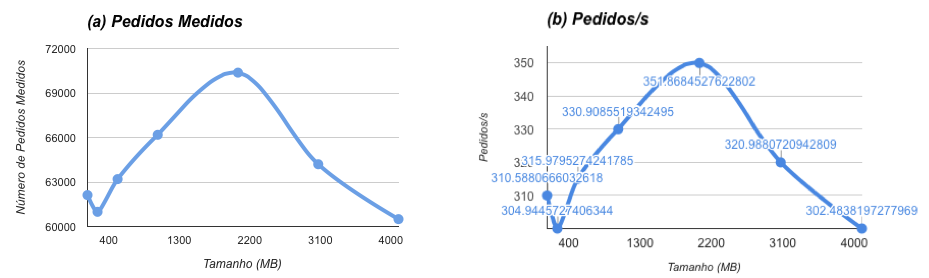
\includegraphics[width=\textwidth]{img/01_sb.png}
\caption{Gráfico correspondente aos valores da tabela anterior\label{overflow}}
\end{figure}

Ao analisar-mos os resultados obtidos, verifica-se que o percentil da latência média e a 99\% estão constantemente a diminuir à medida que a quantidade de memória disponível aumenta. Isto acontece devido à ausência de escrita dos resultados para o disco, o que provoca a redução de quantidade de \textit{I/O} para a obtenção de dados. Conclui-se ainda que o melhor resultado aconteceu quando a memória disponível era de \textbf{2048MB}, tendo ocorrido mais pedidos por segundo e as latências (média e 99\%) apresentarem os resultados mais inferiores. A segunda melhor configuração para esta métrica aconteceu quando a memória disponível era de \textbf{1024MB}.

Assim sendo, para esta configuração o valor escolhido será o de \textbf{2048MB} por apresentar os melhores resultados tanto a nível de pedidos como de latência.

\newpage

\subsection{Configuração \textit{effective\_cache\_size}}

O \textit{effective\_cache\_size} é definido como uma estimativa da quantidade de memória disponível para a \textit{cache} do disco. Este parâmetro é utilizado \textit{PostgreSQL Query Planner} para perceber que planos pode utilizar tendo em conta o espaço disponível em memória.

A documentação do \textit{PostgreSQL} afirma que definir 50\% da memória total do dispositivo será uma configuração conservadora e que 75\% uma configuração agressiva, mas aceitável.

Então para a configuração deste \textit{benchmark} utilizou-se os seguintes parâmetros, 128MB, 512MB, 1024MB, 2048MB, 4096MB e 6144MB.

\begin{table}[!h]
\center
\small
\begin{tabular}{|c|c|c|c|c|}
\hline
\textbf{\# tamanho (MB)} & \textbf{\# pedidos} & \textbf{pedidos/s} & \textbf{lat. média (s)} & \textbf{lat. perct. 99 (s)}  \\ \hline
128 (Default) & 62118 & 310.58806660326184 & 1.022099449909098 & 1.130365  \\ \hline
512 & 67022 & 335.1094363325237 & 1.0208270027602877 & 1.112753  \\ \hline
1024 & 66987 & 334.93426967582496 & 1.0204846512009793 & 1.109516  \\ \hline
2048 & 66478 & 332.38835629969145 & 1.020474478669635 & 1.112206  \\ \hline
4096 & 59880 & 299.3983502432346 & 1.0226386898630595 & 1.131897  \\ \hline
6144 & 63982 & 319.9084020175434 & 1.0210112850958082 & 1.130562  \\ \hline
\end{tabular}
\caption{Resultados obtidos para X (X) armazéns}
\end{table}

\begin{figure}[ht!]
\centering
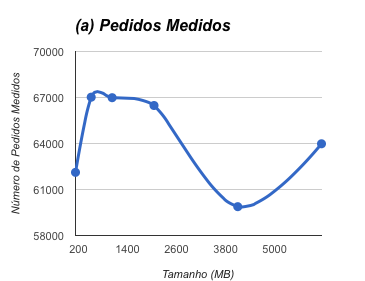
\includegraphics[width=70mm]{img/02_ecs_b.png}
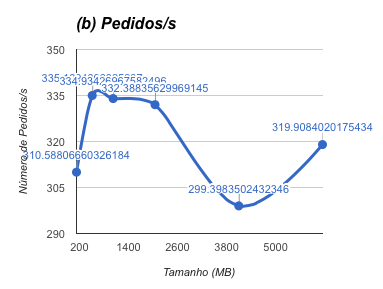
\includegraphics[width=70mm]{img/02_ecs_a.png}
\caption{Gráfico correspondente aos valores da tabela anterior\label{overflow}}
\end{figure}


Ao analisar-se os valores obtidos identificasse que na configuração mais conservadora (\textbf{4096MB}) e agressiva (\textbf{6144MB}) não se obteve os melhores resultados. O número de pedidos medidos foi muito inferior a outros valores assim como a latência a 99\%, a latência média praticamente se encontra entre a média dos resultados.

Podemos, então, definir o intervalo de \textbf{[512-2048]MB} como o que se obteve melhor resultados para esta configuração. O valor \textbf{1024MB} obteve melhor resultados no percentil da lantência a 99\%. Já o valor \textbf{512MB} obteve mais pedidos e pedidos por segundo e um ligeiro aumento nas latências do teste, que influência negativamente o resultado. Com o parâmetro a \textbf{2048MB} mantém-se na média dos resultados anteriores, possuíndo o resultado com menor latência média.

Dentro do intervalo definido anteriormente, se fosse necessário escolher um resultado como melhor valor, escolhíamos a configuração com \textbf{1024MB} de \textit{effective\_cache\_size} onde se obteve a menor latência a 99\% e valor similares na latência média para o praticamente o mesmo número de pedidos.

\newpage

\subsection{Configuração \textit{checkpoint\_segments}}

O \textit{PostgreSQL} escreve novas transações na base de dados em ficheiros chamados de segmentos \textit{Write-Ahead Logging (WAL)} que tem um tamanho de 16MB. Nas configurações do \textit{postgresql.conf} o valor atualmente por defeito é de 3 \textit{checkpoint\_segments}.

Aumentar o número de \textit{checkpoint\_segments} melhora o desempenho do benchmark pois faz com que os \textit{checkpoints} ocorram com menor frequência, obrigando assim a base de dados a uma recuperação mais lenta após uma falha. No entanto o \textit{I/O} ao disco diminui.

Para este \textit{benchmarking} foram utilizados os seguintes valores de \textit{checkpoint\_segments}, 3, 9 e 16.

\begin{table}[!h]
\center
\small
\begin{tabular}{|c|c|c|c|c|}
\hline
\textbf{\# segmentos} & \textbf{\# pedidos} & \textbf{pedidos/s} & \textbf{lat. média (s)} & \textbf{lat. perct. 99 (s)}  \\ \hline
3 (Default) & 62118 & 310.58806660326184 & 1.022099449909098 & 1.130365  \\ \hline
9 & 66254 & 331.26961583822094 & 1.0211749849065717 & 1.113339  \\ \hline
16 & 54564 & 272.81969749069896 & 1.0238594005571438 & 1.103626  \\ \hline
\end{tabular}
\caption{Resultados obtidos para o \textit{checkpoint\_segments}.}
\end{table}

\begin{figure}[ht!]
\centering
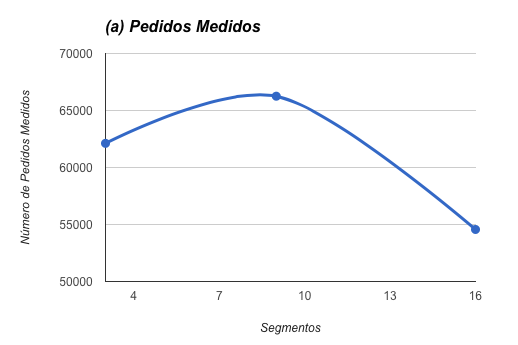
\includegraphics[width=70mm]{img/03_cs_a.png}
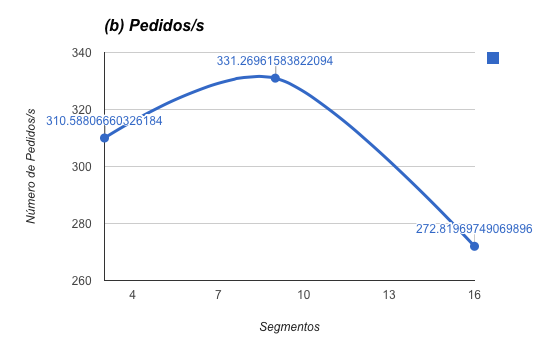
\includegraphics[width=70mm]{img/03_cs_b.png}
\caption{Gráfico correspondente aos valores da tabela anterior\label{overflow}}
\end{figure}

Como foi de esperar, ao aumentar o valor de \textit{checkpoint\_segments} o valores de transações aumentaram, mas somente quando o valor foi de 9 segmentos. Quando o teste foi efetuado com \textbf{16} segmentos o número de transações dimininuiram abruptamente mas na latência a 99\% obteve-se o melhor resultado, ainda que na latência média manteve-se perto dos resultados anteriores. Estes resultados podem-se dever à recuperação mais lenta da base de dados.

Nesta situação a configuração mais indicada seria de \textbf{9} segmentos. O \textit{benchmark} obteve o melhore resultado ao nível das transações e de latência média inferior nestas transações.

Normalmente para valores elevados de \textit{checkpoint\_segments} é recomendado aumentar o \textit{checkpoint\_timeout} por causa dos intervalos de controlo.

\newpage

\subsection{Configuração \textit{autovacuum\_naptime}}

Este processo corresponde ao tempo mínimo entre a execução do \textit{autovacuum}, isto é, só ocorre um novo depois de ter passado o tempo de execução do anterior.

Para perceber o que acontece nesta configuração foram feitos vários \textit{benchmarks} para os seguintes tempos de \textit{autovacuum\_naptime}: desligado, 1 minuto, 2 minutos e 3 minutos entre cada execução. Obteve-se, assim, os resultados da próxima tabela.

\begin{table}[!h]
\center
\small
\begin{tabular}{|c|c|c|c|c|}
\hline
\textbf{\# tempo (min)} & \textbf{\# pedidos} & \textbf{pedidos/s} & \textbf{lat. média (s)} & \textbf{lat. perct. 99 (s)}  \\ \hline
0 (off) & 59802 & 299.0081276096099 & 1.021858928530818 & 1.136963  \\ \hline
1 (Default) & 62118 & 310.5880666032618 & 1.022099449909098 & 1.130365  \\ \hline
2 & 53296 & 266.4799488385146 & 1.025329163370609 & 1.138289  \\ \hline
3 & 61163 & 305.8148124055486 & 1.022736959518009 & 1.124206  \\ \hline
\end{tabular}
\caption{Resultados obtidos para a configuração do \textit{autovacuum\_naptime}}
\end{table}

\begin{figure}[ht!]
\centering
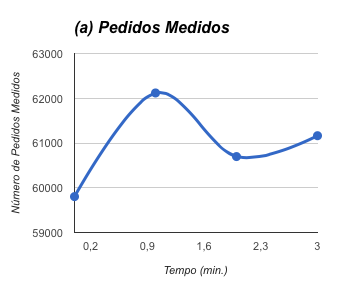
\includegraphics[width=70mm]{img/05_vacuum_a.png}
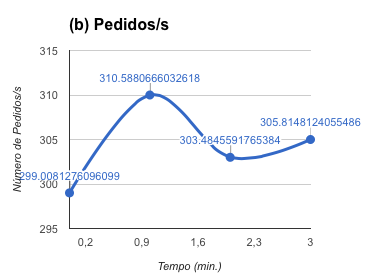
\includegraphics[width=70mm]{img/05_vacuum_b.png}
\caption{Gráficos correspondente aos valores da tabela \label{overflow}}
\end{figure}

Dos resultados apresentados, verifica-se que, os que apresentam melhores tempos de execução foram o de \textbf{1} minuto e \textbf{3} minutos. Este último só ocorreu no máximo uma vez, assim como o teste a \textbf{2} minutos, o que leva a querer que não teve muita influência nos valores da latência. Com o parâmetro desligado não se obteve os resultados mais corretos, isto porque não ocorreu nenhuma execução do \textit{\textbf{autovacuum}} o que contribui para estatísticas erradas e consequentemente para escolha errada dos algoritmos usados pelo \textit{PostgreSQL}.

Ao contrário do esperado ter um \textit{\textbf{autovacuum}} mais regular fez que os resultados obtidos fossem mais razoáveis com os que se pode comparar. De facto, ao haver com mais frequência o \textit{\textbf{autovacuum}} faz com que em cada operação haja menos dados para limpar.

Assim, decidiu-se escolhar para esta configuração o melhor resultado o de \textbf{1} minuto, por defeito na configuração do \textit{postgresql.conf}.

\newpage

\subsection{Configuração \textit{work\_mem}}

O \textit{work\_mem} especifica a quantidade de memória RAM que pode ser usada para operações internas (\textit{Sort e Hash Tables}) antes de serem gravadas para ficheiros temporários em disco. O valor predefinido na configuração do \textit{PostgreSQL} é de 1MB.

Como existem algumas \textit{queries} complexas no teste do \textit{CHBenchmark} decidimos testar como vão variar o tempo de execução das \textit{queries} e perceber se é possível obter mais transações com a menor latência possível. Para isto foram feitos testes para 1MB, 8MB, 32MB, 128MB e 512MB.

\begin{table}[!h]
\center
\small
\begin{tabular}{|c|c|c|c|c|}
\hline
\textbf{\# tamanho (MB)} & \textbf{\# pedidos} & \textbf{pedidos/s} & \textbf{lat. média (s)} & \textbf{lat. perct. 99 (s)}  \\ \hline
1 (Default) & 62118 & 310.5880666032618 & 1.022099449909098 & 1.130365  \\ \hline
8 & 62391 & 311.9513589177765 & 1.021819045423218 & 1.130889  \\ \hline
32 & 67109 & 335.5443187426919 & 1.019860019833405 & 1.117067  \\ \hline
128 & 67728 & 338.6382522575026 & 1.018854204671627 & 1.118497  \\ \hline
512 & 67698 & 338.4895027961542 & 1.020378764261869 & 1.118507  \\ \hline
\end{tabular}
\caption{Resultados obtidos para X (X) armazéns}
\end{table}

\begin{figure}[ht!]
\centering
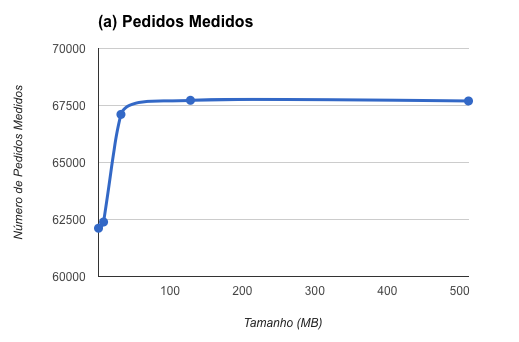
\includegraphics[width=70mm]{img/06_wm_a.png}
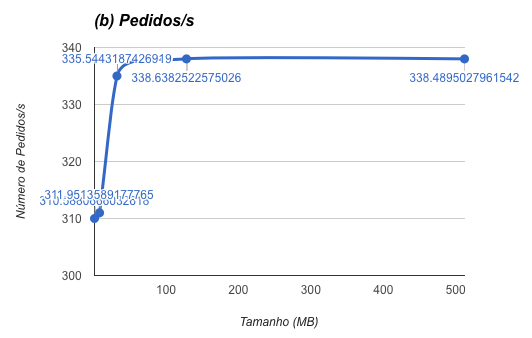
\includegraphics[width=70mm]{img/06_wm_b.png}
\caption{Gráficos correspondente aos valores da tabela \label{overflow}}
\end{figure}

Através das ferramentas que acompanham o \textit{oltpbench}, nomeadamente o \textit{plot\_latencies.py} obtivemos o seguinte gráfico, para os valores médios de execução:

\begin{figure}[ht!]
\centering
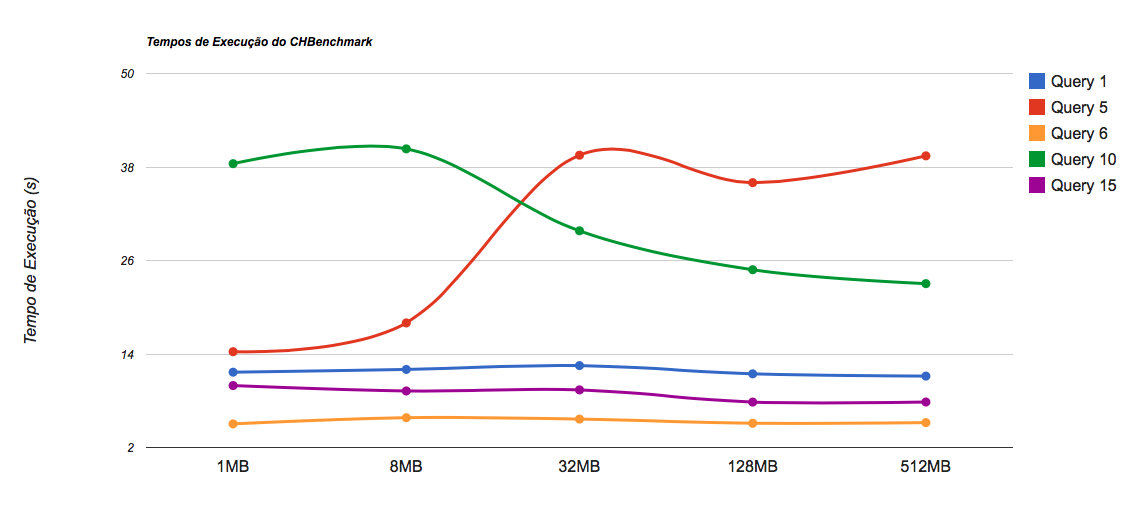
\includegraphics[width=\textwidth]{img/06_wm_c.png}
\caption{Gráfico com os valores de execução para cada query com diferentes valores de memória\label{overflow}}
\end{figure}

Como verificámos no gráfico anterior o tempo de execução variou significativamente em duas \textit{queries}, na \textit{Query 10} que tinha um tempo de execução superior na configuração inicial e que passou a obter um tempo de execução inferior, proporcionalmente à memória disponível. Já na \textit{Query 17} que inicialmente tinha um tempo de execução inferior passou a tempos muitos superiores ao esperado. Isto deve-se ao facto dos algoritmos escolhidos terem efeito na quantidade de memória definida.

Os resultados das \textit{queries 1, 6 e 17} os resultados praticamente não surtiram grande variação nos resultados.

Caso fosse necessário escolher a melhor configuração para este parâmetro, este ficaria entre os \textbf{8MB e 32MB}. Será necessário efetuar mais um teste, por exemplo, com \textbf{16MB} para perceber se houve alguma alteração na execução das \textit{queries} que tire partido deste valor.

Finalmente, se analisar-mos o valor das latências junto com as transações medidas, percebe-se que \textbf{32MB} será provavelmente uma boa configuração para este parâmetro.


\subsection{Configuração do \textit{random\_page\_cost}}

Como o dispositivo utilizado para correr os testes possui um \textit{Solid State Drive (SSD)} decidou-se alterar na configuração do \textit{PostgreSQL} o custo dos acessos aleatórios. Neste teste vamos mostrar os resultados obtidos para a configuração inicial que tem definido um custo igual a 4, e alterações de custo entre 1 e 2.

\begin{table}[!h]
\center
\small
\begin{tabular}{|c|c|c|c|c|}
\hline
\textbf{\# custo} & \textbf{\# pedidos} & \textbf{pedidos/s} & \textbf{lat. média (s)} & \textbf{lat. perct. 99 (s)}  \\ \hline
4.0 (Default) & 62118 & 310.58806660326184 & 1.022099449909098 & 1.130365  \\ \hline
2.0 & 65295 & 326.47479814226466 & 1.0193406799754958 & 1.116984  \\ \hline
1.0 & 58540 & 292.69854964502616 & 1.0225425792791254 & 1.133753  \\ \hline
\end{tabular}
\caption{Resultados obtidos para 3 tipos diferentes de custos}
\end{table}

\begin{figure}[ht!]
\centering
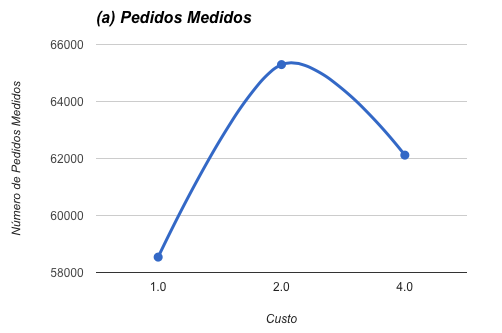
\includegraphics[width=70mm]{img/07_rpc_a.png}
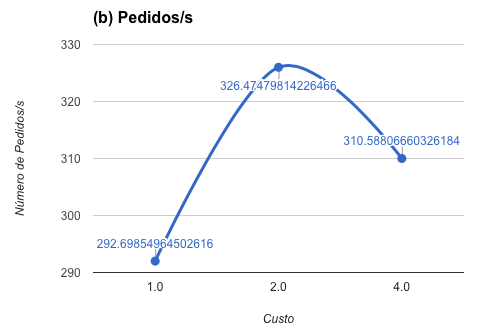
\includegraphics[width=70mm]{img/07_rpc_b.png}
\caption{Gráficos correspondente aos valores da tabela \label{overflow}}
\end{figure}

Da análise dos resultados obtidos nas tabelas e gráficos verifica-se que se o custo dos acessos aleatórios for de \textbf{2} encontram-se melhores valores de latência média e a 99\%. Também o número de pedidos medios por tempo é superior ao definido por defeito na configuração inicial.

De notar, que quando o custo é de \textbf{1} os valores são muito inferiores aos desejados.

Conclui-se então que se diminuir o custo dos acessos aleatórios para \textbf{2} irá beneficiar a execução do \textit{benchmark}. Isto acontece porque a escolha do algoritmo vai passar a optar em algumas partes da \textit{query} por usar acessos aleatórios em vez dos preteridos acessos sequenciais.

\newpage

\subsection{Configuração do \textit{shared\_buffers} com o \textit{effective\_cache\_size}}

Escolhida a melhor configurações do \textit{shared\_buffers}, o intervalo de mémoria [1024-2048]MB. No \textit{effective\_cache\_size} decidiu-se usar o melhor resultado da configuração anterior, 1024MB, e testar, também, os valores de memória conservadora e agressiva definidos anteriormente, 4096MB e 6144MB, respectivamente.

Os resultados obtidos para esta configuração são os seguintes:

\begin{table}[!h]
\center
\small
\begin{tabular}{|c|c|c|c|c|}
\hline
\textbf{\# tamanho} & \textbf{\# pedidos} & \textbf{pedidos/s} & \textbf{lat. perct. média} & \textbf{lat. perct. 99}  \\ \hline
1024MB & 69015 & 345.073418193803 & 1.02032663525321 & 1.094924  \\ \hline
4096MB & 67377 & 336.882924828134 & 1.02042478753877 & 1.095611  \\ \hline
6144MB & 65443 & 327.214804387718 & 1.02116393962685 & 1.092516  \\ \hline
\end{tabular}
\caption{Resultados obtidos para o valor de 1024MB de \textit{shared\_buffers}}
\end{table}

\begin{table}[!h]
\center
\small
\begin{tabular}{|c|c|c|c|c|}
\hline
\textbf{\# tamanho} & \textbf{\# pedidos} & \textbf{pedidos/s} & \textbf{lat. perct. média} & \textbf{lat. perct. 99}  \\ \hline
1024MB & 74724 & 373.619008187245 & 1.01803675496494 & 1.088794  \\ \hline
4096MB & 66985 & 334.923957423586 & 1.01998354016571 & 1.112503  \\ \hline
6144MB & 69708 & 348.538465057512 & 1.01924645791014 & 1.095748  \\ \hline
\end{tabular}
\caption{Resultados obtidos para o valor de 2048MB de \textit{shared\_buffers}}
\end{table}

\begin{figure}[ht!]
\centering
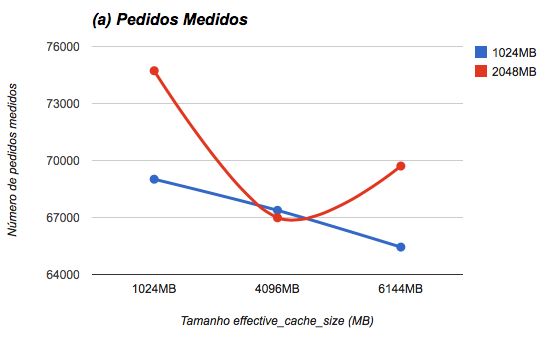
\includegraphics[width=70mm]{img/questao_3/sb_ecs_a.png}
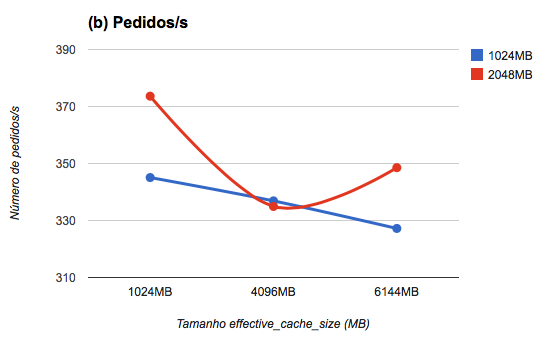
\includegraphics[width=70mm]{img/questao_3/sb_ecs_b.png}
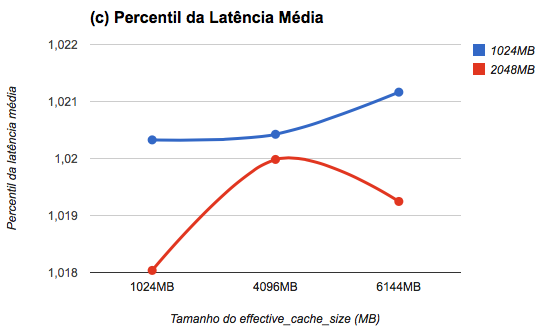
\includegraphics[width=70mm]{img/questao_3/sb_ecs_c.png}
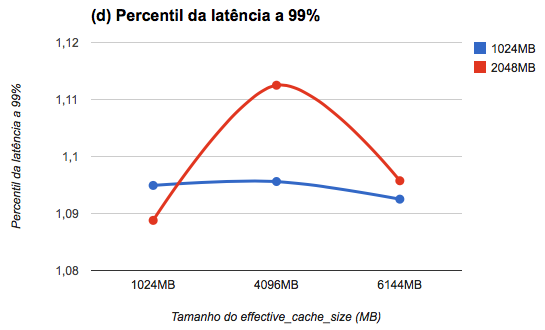
\includegraphics[width=70mm]{img/questao_3/sb_ecs_d.png}
\caption{Gráficos corresponde às variações do \textit{shared\_buffers} para cada \textit{effective\_cache\_size}}
\end{figure}

Desta vez, consegui-se perceber que a configuração mais agressiva do \textit{effective\_cache\_size} (\textbf{6144MB}) teve melhores resultados neste \textit{benchmark} dos que nos resultados indivuais do parâmetro.

Conclui-se facilmente que a melhor configuração obtida foi de \textbf{6144MB}  de \textit{shared\_buffers} e de \textbf{1024MB} de \textit{effective\_cache\_size}. Através da análise dos gráficos verifica-se que se obteve mais pedidos por segundo e o percentil das latências (média e a 99\%) são os mais baixos. Esta configuração será mantida para a próxima configuração.

Desta forma, percebe-se que ter muita quantidade de memória RAM disponível não significa que se vai obter resultados com qualidade superior, antes pelo contrário, como provado neste \textit{benchmark}.

\subsection{Configuração anterior com o \textit{checkpoint\_segments}}

\begin{table}[!h]
\center
\small
\begin{tabular}{|l|c|}
\hline
\textbf{Parâmetro} & \textbf{Valor} \\ \hline
\textbf{shared\_buffers} & 2048MB  \\ \hline
\textbf{effective\_cache\_size} & 1024MB  \\ \hline
\end{tabular}
\end{table}

Assim para os melhores resultados obtidos na configuração individual do \textit{checkpoint\_segments}, 3 e 9 segmentos, vamos testar estes valores com a configuração definida na tabela anterior.

\begin{table}[!h]
\center
\small
\begin{tabular}{|c|c|c|c|c|}
\hline
\textbf{\# segmentos} & \textbf{\# pedidos} & \textbf{pedidos/s} & \textbf{lat. média (s)} & \textbf{lat. perct. 99 (s)}  \\ \hline
3Segmentos & 74724 & 373.619008187245 & 1.01803675496494 & 1.088794  \\ \hline
9Segmentos & 75410 & 377.048437684716 & 1.01657169486805 & 1.085938  \\ \hline
\end{tabular}
\caption{Resultados com variações do número de segmentos}
\end{table}

\begin{figure}[ht!]
\centering
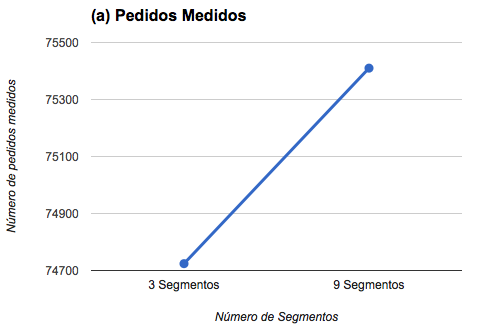
\includegraphics[width=70mm]{img/questao_3/sb_ecs_cs_a.png}
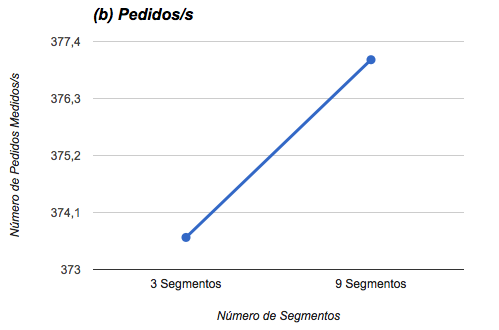
\includegraphics[width=70mm]{img/questao_3/sb_ecs_cs_b.png}
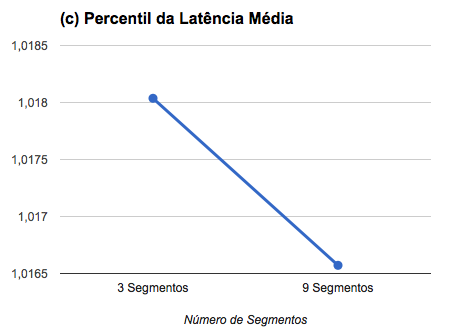
\includegraphics[width=70mm]{img/questao_3/sb_ecs_cs_c.png}
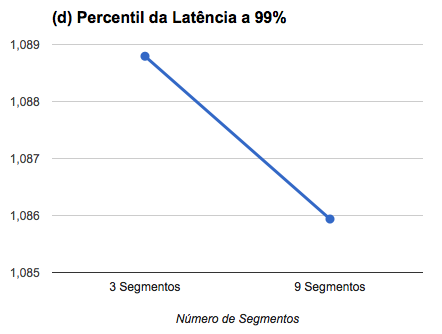
\includegraphics[width=70mm]{img/questao_3/sb_ecs_cs_d.png}
\caption{Gráficos corresponde às variações das configurações anteriores com \textit{checkpoint\_segments}}
\end{figure}

Como esperado o aumento do número de \textit{checkpoint\_segments} permitiu aumentar o número de transações medidas e diminuir as latências (média e a 99\%).

Assim para a próxima configuração será usado um \textit{checkpoint\_segments} de 9 segmentos. De notar que apesar deste aumento significativo dos resultados o tempo de recuperação da Base de Dados será mais lento.


\newpage

\subsection{Configuração anterior com o \textit{autovacuum\_naptime}}

\begin{table}[!h]
\center
\small
\begin{tabular}{|l|c|}
\hline
\textbf{Parâmetro} & \textbf{Valor} \\ \hline
\textbf{shared\_buffers} & 2048MB  \\ \hline
\textbf{effective\_cache\_size} & 1024MB  \\ \hline
\textbf{checkpoint\_segments} & 9 Segmentos \\ \hline
\end{tabular}
\end{table}

Como na configuração individual do \textit{autovacuum\_naptime} não se obteve resultados razoáveis para 2 e 3 minutos, decidiu-se para este teste efetuar novos tempos de execução do \textit{autovacuum}. Assim serão usados 30, 60 (predefinido) e 90 segundos neste \textit{benchmark}.

Com a configuração da tabela anterior mais os novos parâmetros definidos obteve-se os seguintes resultados, representados na seguinte tabela e nos próximos gráficos.

\begin{table}[!h]
\center
\small
\begin{tabular}{|c|c|c|c|c|}
\hline
\textbf{\# tempos} & \textbf{\# pedidos} & \textbf{pedidos/s} & \textbf{lat. média (s)} & \textbf{lat. perct. 99 (s)}  \\ \hline
30Segundos & 76469 & 382.342824656676 & 1.01569113987367 & 1.088295  \\ \hline
60Segundos & 75410 & 377.048437684716 & 1.01657169486805 & 1.085938  \\ \hline
90Segundos & 74100 & 370.498798459429 & 1.0184869048448 & 1.089411  \\ \hline
\end{tabular}
\caption{Resultados obtidos para diferentes tempos de \textit{autovacuum\_naptime}}
\end{table}

\begin{figure}[ht!]
\centering
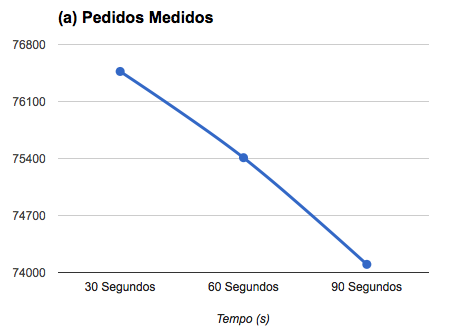
\includegraphics[width=70mm]{img/questao_3/sb_ecs_cs_vacuum_a.png}
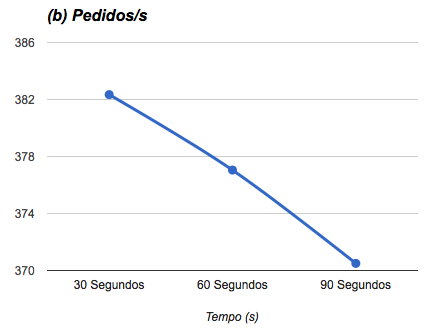
\includegraphics[width=70mm]{img/questao_3/sb_ecs_cs_vacuum_b.png}
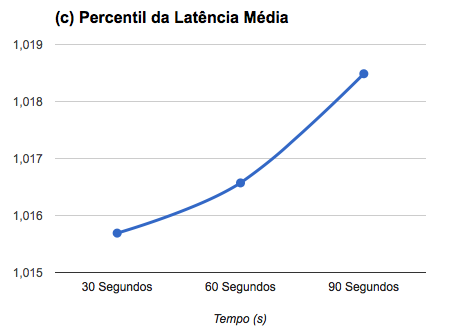
\includegraphics[width=70mm]{img/questao_3/sb_ecs_cs_vacuum_c.png}
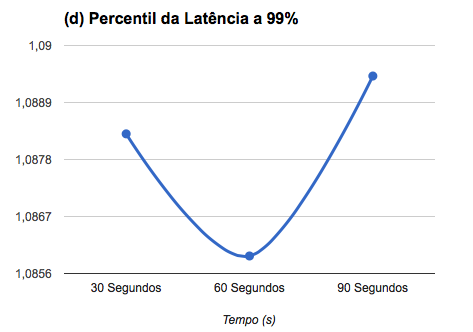
\includegraphics[width=70mm]{img/questao_3/sb_ecs_cs_vacuum_d.png}
\caption{Corresponde às variações das configurações anteriores com \textit{autovacuum\_naptime}}
\end{figure}

A partir dos resultados acima demonstrados verifica-se que o melhor resultado aconteceu quando o tempo de \textbf{30} segundos estava definido. Como verificado, com o aumento do valor do \textit{autovacuum\_naptime} nota-se, perfeitamente, que os resultados pioraram de forma significativa.

Como tal na próxima configuração o valor do \textit{autovacuum\_naptime} será de \textbf{30} segundos.

\newpage

\subsection{Configuração anterior com o \textit{random\_page\_cost}}

\begin{table}[!h]
\center
\small
\begin{tabular}{|l|c|}
\hline
\textbf{Parâmetro} & \textbf{Valor} \\ \hline
\textbf{shared\_buffers} & 2048MB  \\ \hline
\textbf{effective\_cache\_size} & 1024MB  \\ \hline
\textbf{checkpoint\_segments} & 9 Segmentos \\ \hline
\textbf{autovacuum\_naptime} & 30 Segundos \\ \hline
\end{tabular}
\end{table}

\newpage

\subsection{Configuração anterior com o \textit{work\_mem}}

\begin{table}[!h]
\center
\small
\begin{tabular}{|l|c|}
\hline
\textbf{Parâmetro} & \textbf{Valor} \\ \hline
\textbf{shared\_buffers} & 2048MB  \\ \hline
\textbf{effective\_cache\_size} & 1024MB  \\ \hline
\textbf{checkpoint\_segments} & 9 Segmentos \\ \hline
\textbf{autovacuum\_naptime} & 30 Segundos \\ \hline
\textbf{work\_mem} & xxMB \\ \hline
\end{tabular}
\end{table}

